\documentclass[submit]{harvardml}

\course{CS181-S21}
\assignment{Assignment \#3}
\duedate{7:59pm EST, March 5, 2021}

\usepackage[OT1]{fontenc}
\usepackage[colorlinks,citecolor=blue,urlcolor=blue]{hyperref}
\usepackage[pdftex]{graphicx}
\usepackage{subfig}
\usepackage{fullpage}
\usepackage{amsmath}
\usepackage{amssymb}
\usepackage{color}
\usepackage{soul}
\usepackage{todonotes}
\usepackage{listings}
\usepackage{common}
\usepackage{enumitem}
\usepackage{bm}
\usepackage{float}
\newcommand{\B}{\text{B}}
\newcommand{\Beta}{\text{Beta}}


\usepackage{xcolor}
\definecolor{deepblue}{rgb}{0,0,0.5}
\definecolor{deepred}{rgb}{0.6,0,0}
\definecolor{deepgreen}{rgb}{0,0.5,0}
 
\lstset{
    language=Python, 
    basicstyle=\ttfamily\small, 
    keywordstyle=\color{deepblue},
    commentstyle=\color{deepgreen},
    stringstyle=\color{deepgreen},
    showstringspaces=false,
    frame=tb,
    identifierstyle=\color{deepred}
    }

\usepackage[mmddyyyy,hhmmss]{datetime}

\definecolor{verbgray}{gray}{0.9}

\lstnewenvironment{csv}{%
  \lstset{backgroundcolor=\color{verbgray},
  frame=single,
  framerule=0pt,
  basicstyle=\ttfamily,
  columns=fullflexible}}{}

\begin{document}

\begin{center}
{\Large Homework 3: Bayesian Methods and Neural Networks}\\
\end{center}

\subsection*{Introduction}

This homework is about Bayesian methods and Neural Networks.  Section 2.9 in the textbook as well as reviewing MLE and MAP will be useful for Q1. Chapter 4 in the textbook will be useful for Q2.

Please type your solutions after the corresponding problems using this
\LaTeX\ template, and start each problem on a new page.

Please submit the \textbf{writeup PDF to the Gradescope assignment `HW3'}. Remember to assign pages for each question.  \textbf{All plots you submit must be included in your writeup PDF.  }We will not be checking your code / source files except in special circumstances. 

Please submit your \textbf{\LaTeX file and code files to the Gradescope assignment `HW3 - Supplemental'}. 


\begin{problem}[Bayesian Methods]

  This question helps to build your understanding of making
  predictions with a maximum-likelihood estimation (MLE), a maximum a
  posterior estimator (MAP), and a full posterior predictive.

  Consider a scalar variable $x$ with the following generative
  process: First, the mean $\mu$ is sampled from a prior
  $N(0,\tau^2)$.  Next, each $x_n$ is generated as $x_n = \mu +
  \epsilon_n$, where $\epsilon_n \sim N(0,\sigma^2)$. All
  $\epsilon_n$'s are independent of each other and of $\mu$.

  For this problem, use $\sigma^2 = 1$ and $\tau^2 = 5$.  

  Now, we see 14 independent samples of $x$ to yield data
  $$D = 3.3, 3.5, 3.1, 1.8, 3.0, 0.74, 2.5, 2.4, 1.6, 2.1, 2.4, 1.3, 1.7, 0.19$$
    
  \textit{Make sure to include all required plots in your PDF.}

\begin{enumerate}

\item Derive the expression for $p(\mu|D)$.  Do \emph{not} plug in
  numbers yet!

  Hint: Use properties of normal-normal conjugacy to simplify your derivation.  You can also refer to \href{https://www.cs.ubc.ca/~murphyk/Papers/bayesGauss.pdf}{this paper}.
  
\item Now we get to our core interest: the predictive distribution of
  a new datapoint $x^*$ given our observed data $D$, $p(x^*|D)$.
  Write down the expression for the full posterior predictive
  distribution: $$p(x^*|D) = \int p(x^*|\mu)p(\mu|D) d\mu$$ Interpret
  your expression in a few words.  Do \emph{not} plug in numbers yet!

  Hint: To simplify your derivation,
  use the fact that $x = \mu + \epsilon$, and $\mu|D$ and $\epsilon$
  are independent Gaussians whose distributions you know from above.
  
\item The full posterior predictive distribution had a nice analytic
  form in this case, but in many problems, it is often difficult to
  calculate because we need to marginalize out the parameters (here,
  the parameter is $\mu$). We can mitigate this problem by plugging in
  a point estimate of $\mu^*$ rather than a distribution. Derive the
  estimates of $p(x^*|D) \approx p(x^*|\mu^*)$ for $\mu^* = \mu_{MLE}$
  and $\mu^* = \mu_{MAP}$.  How do these expressions compare to the
  expression for the full posterior above? Do \emph{not} plug in
  numbers yet!
  
   
\item Plot how the above 3 distributions change after each data point
  is gathered.  You will have a total of 15 plots, starting with the
  plot for the case with no data (they can be small, e.g. in a $3\times5$
  grid).  The x-axis of each plot will be the $x$ value and the y-axis
  the density.  You can make one plot for each estimator, or combine
  all three estimators onto one plot with a different colored line for
  each estimator.
  
    
\item How do the means of the predictive distributions vary with more
  data?  How do the variances vary?  Interpret the differences you see
  between the three different estimators.
  
  \item Does the ordering of the data matter for the final predictive
  distributions?  

  \item Derive an expression for and then compute the marginal
    likelihood of the training data $p(D)$.

    Hint: You can rearrange the required integral such that it looks like an un-normalized
    Gaussian distribution in terms of $\mu$,  and take advantage of the fact that
    integrating over a normalized Gaussian distribution is equal to 1.
    You will need to complete the square.
    
  \item Now consider an alternate model in which we were much more sure
  about the mean: $\mu \sim N(0,\tau^2)$, where $\tau^2 = 0.1$.
  Compute the marginal likelihood $p(D)$ for this model.  Which of the
  two models has a higher marginal likelihood? Interpret this result.

\end{enumerate}

\end{problem}

\subsection*{Solution 1:}

\begin{enumerate}
    \item \textbf{Derive the expression for $p(\mu | D)$}.\\ \\
    The question defines $\sigma^2 = 1$ and $\tau^2 = 5$, we can use this information to define $\sigma_0^2 = 5$ and $\mu_0 = 0$ when using the syntax of the referenced paper.
    Using the properties of normal-normal conjugacy from the referenced paper we can derive and simplify the following:
    $$
        p(\mu | D) \propto p(D | \mu)p(\mu | \mu_0,\sigma_0^2)
    $$
    $$
        p(\mu|D) \propto exp \left[ \frac{-1}{2\sigma^2} \sum_i (x_i^2 + \mu^2 - 2 x_i \mu) + \frac{-1}{2\sigma^2} (\mu^2 + \mu_0^2 - 2\mu_0 \mu) \right]
    $$
    $$
        \mu_n = \frac{1}{\frac{1}{\sigma_0^2} + \frac{n}{\sigma^2}} \left( \frac{\mu_0}{\sigma_0^2} + \frac{\sum^n_{i=1} x_i}{\sigma^2} \right)
    $$
    
    $$
        \sigma_n^2 = \left( \frac{1}{\sigma_0^2} + \frac{n}{\sigma^2} \right)^{-1}
    $$
    \item \textbf{Write down the expression for the full posterior predictive distribution $p(x* | D)$:}\\
    
    As $x = \mu + \epsilon$ and $\epsilon_n \sim N(0,\sigma^2)$, $\mu |D \sim N(\mu_n, \sigma_n)$ 
    
    \begin{align*}
        p(x^*|D) &= \int p(x^*|\mu)p(\mu|D) d\mu \\
        &= \int \mathcal{N} (x*|\mu_n , \sigma^2) \mathcal{N} (\mu | \mu_n, \sigma_n^2) d\mu \\
        &= \mathcal{N} (x*|\mu_n , \sigma^2_n + \sigma^2)
    \end{align*}
    Using the linearity of expectation and variance if $X_1$ and $X_2$ are independent, we can see that the result will still be normal - therefore we can just plug into the normal PDF:
    
    $$
        X \sim \mathcal{N} (x*|\mu_n , \sigma^2_n + \sigma^2)
    $$
    
    $$
        p(x* |D) = \frac{1}{\sqrt{2 \pi (\sigma^2_n + \sigma^2)}} e^{ \frac{-1}{2 (\sigma^2_n + \sigma^2)}(x - \mu_n)^2 } 
    $$
    
    \item \textbf{Derive the estimates of $p(x^*|D) \approx p(x^*|\mu^*)$ for $\mu^* = \mu_{MLE}$ and $\mu^* = \mu_{MAP}$}
    
    At each step through $D$we are using a $\mu* = \mu_{MLE}$ or $\mu* = \mu_{MAP}$ respectively for each.
    
    We can first derive the expression of $\mu_{MLE}$:
    \begin{align*}
        P(D | \mu) &= \prod^N_{i=1} \frac{1}{\sqrt{2 \pi \sigma^2}} e ^{- \frac{(x_i - \mu)^2}{2\sigma^2}}
    \end{align*}
    Now we can take the log to simplify:
    \begin{align*}
        \log{P(\mu | D)} = \sum^N_{i=1} \log(\frac{1}{\sqrt{2 \pi \sigma^2}}) {- \frac{(x_i - \mu)^2}{2\sigma^2}}
    \end{align*}
    Taking the derivative:
    \begin{align*}
        \frac{\partial \log{P(\mu | D)}}{\partial \mu} &= \sum^N_{i=1}  - (-2) \frac{(x_i - \mu)^2}{2\sigma^2} \\
        &= \sum^N_{i=1}  \frac{(x_i - \mu)}{\sigma^2} = 0 \\
        0 &= \sum^N_{i=1} (x_i) - N\mu \\
        \hat{\mu}_{MLE} &= \frac{\sum^N_i x_i}{N}
    \end{align*}
    
    We can similarly derive the expression of $\mu_{MAP}$:
    \begin{align*}
        P(\mu | D) &= \frac{P(D| \mu) PD\mu}{P(D)}\\
        P(D | \mu) &= \prod^N_{i=1} \frac{1}{\sqrt{2 \pi \sigma^2}} e ^{- \frac{(x_i - \mu)^2}{2\sigma^2}}
    \end{align*}
    
    We are given that the $\sigma^2$ of $\mu$ is $\tau^2$:
    \begin{align*}
         P(\mu) = \frac{1}{\sqrt{2 \pi \tau^2}} e ^{- \frac{(x_i - \mu)^2}{2\tau^2}}
    \end{align*}
    Plugging this into the equation above for $P(\mu | D)$ and the equation for $P(D | \mu)$ from the previous question we have:
    
    \begin{align*}
        P(\mu | D) &= \frac{ \left( \prod^N_{i=1} \frac{1}{\sqrt{2 \pi \sigma^2}} e ^{- \frac{(x_i - \mu)^2}{2\sigma^2}} \right) \frac{1}{\sqrt{2 \pi \tau^2}} e ^{- \frac{(x_i - \mu)^2}{2\tau^2}} }{P(D)}
    \end{align*}
    Taking logs and differentiating to find the maximising $\mu$
    
    \begin{align*}
        \frac{\partial \log (P(\mu | D)}{\partial \mu} & = \left( \sum^N_i \frac{x_i - \mu}{\sigma^2}\right) - \frac{\mu - \mu_0}{\tau^2} = 0 \\
        \frac{\mu - \mu_0}{\tau^2} &= - \frac{\sigma^N_i x_i}{\sigma^2} - \frac{N\mu}{\sigma^2} \\
        \hat{\mu}_{MAP} &= \frac{\sigma^2 \mu_0 + \tau^2 \sum _i^N x_i}{\sigma^2 + N\tau^2}
    \end{align*}
    
    $\hat{\mu}_{MAP}$ differs to $\hat{\mu}_{MLE}$ in that it takes into account the posterior distribution. $\hat{\mu}_{MLE}$ is a special case of the $\hat{\mu}_{MAP}$ in which the posterior is uniform. $\hat{\mu}_{MAP}$ is case of the full posterior where we are integrating only over the models that maximise $\mu$.
    
    \item \textbf{Plot how the above 3 distributions change after each data point is gathered}
    \item \textbf{How do the means of the predictive distributions vary with more data?  How do the variances vary?  Interpret the differences you see between the three different estimators.}
    
    The means of the data do not vary much with additions of new data, the variance will start decreasing as the N increases. 
    
    \item \textbf{Does the ordering of the data matter for the final predictive
  distributions?}
    
    When the N is small the order of the data matters - if skewed data is presented first the estimators will start at a completely different place, however, once you get the end of the dataset it will make no difference as each datapoint will be taken into account. As MLE and MAP and the full posterior use the means to calculate, and the mean at the end will be the same.
  
    \item \textbf{Derive an expression for and then compute the marginal likelihood of the training data $p(D)$: }
    
    \begin{align*}
        P(D) &= \int \prod_i^N  \mathcal{N} (x_i|\mu , \sigma^2) \mathcal{N} (\mu | \mu_0, \tau^2) d\mu \\
        &= \frac{\sigma}{(\sqrt{2\pi \sigma^2})^n \sqrt{n\tau^2 + \sigma^2}} \\
        &= \left(\frac{1}{\sqrt{2\pi \sigma^2}}\right)^n \left(\frac{\sigma}{\sqrt{n\tau^2 + \sigma^2}} \right) \\
    \end{align*}
    
    Plugging in $\sigma^2 = 1$, $n = 14$:
    \begin{align*}
        &= \exp \left[-\frac{1}{2} \left( \sum_{(x \in D)} x_i^2 - \frac{(\sum_{(x \in D)} x_i)^2}{14 + \frac{1}{\tau^2}} \right) \right] \left(\frac{1}{\sqrt{2\pi}}\right)^{14} \left(\frac{1}{\sqrt{1 + 14\tau^2}} \right)
    \end{align*}
    
    Now we can use the datapoints from $D$ to find $\sum_i^N x_i = 29.63$ and $\sum_i^N x_i = 74.8937$ as well as $\tau^2=5$. Plugging this in we can find:
    \begin{align*}
        &= \exp \left[-\frac{1}{2} \left( 74.8937 - \frac{(29.63)^2}{14 + \frac{1}{5}} \right) \right] \left(\frac{1}{\sqrt{2\pi}}\right)^{14} \left(\frac{1}{\sqrt{1 + 14 \times 5}} \right)
    \end{align*}
    This gives a result of: 4.46287266201e-10\\ 
    \item\textbf{ Now consider an alternate model in which we were much more sure about the mean: $\mu \sim N(0,\tau^2)$, where $\tau^2 = 0.1$. Compute the marginal likelihood $p(D)$ for this model.  Which of the two models has a higher marginal likelihood?}
  
  \begin{align*}
        &= \exp \left[-\frac{1}{2} \left( 74.8937 - \frac{(29.63)^2}{14 + \frac{1}{0.1}} \right) \right] \left(\frac{1}{\sqrt{2\pi}}\right)^{14} \left(\frac{1}{\sqrt{1 + 14 \times 0.1}} \right)
    \end{align*}
    Computing this we get 7.999704e-15.
    
    This actually has a lower likelihood result, although this makes sense as a lower $\tau$ will cause the exponent to decay faster.
\end{enumerate}

\newpage
\begin{problem}[Neural Net Optimization]

  In this problem, we will take a closer look at how gradients are calculated for backprop with a simple multi-layer perceptron (MLP). The MLP will consist of a first fully connected layer with a sigmoid activation, followed by a one-dimensional, second fully connected layer with a sigmoid activation to get a prediction for a binary classification problem. Assume bias has not been merged. Let:
  \begin{itemize}
      \item $\bold{W}_1$ be the weights of the first layer, $\bold{b}_1$ be the bias of the first layer.
      \item $\bold{W}_2$ be the weights of the second layer, $\bold{b}_2$ be the bias of the second layer.
  \end{itemize}
  
  The described architecture can be written mathematically as: $$\hat{y} = \sigma(\bold{W}_2 \left[\sigma \left(\bold{W}_1 \bold{x} + \bold{b}_1\right)\right] + \bold{b}_2)$$
  
  where $\hat{y}$ is a scalar output of the net when passing in the single datapoint $\bold{x}$ (represented as a column vector), the additions are element-wise additions, and the sigmoid is an element-wise sigmoid.
  
  \begin{enumerate}
      \item Let:
      \begin{itemize}
          \item $N$ be the number of datapoints we have
          \item $M$ be the dimensionality of the data
          \item $H$ be the size of the hidden dimension of the first layer. Here, hidden dimension is used to describe the dimension of the resulting value after going through the layer. Based on the problem description, the hidden dimension of the second layer is 1.
      \end{itemize}
      
      Write out the dimensionality of each of the parameters, and of the intermediate variables:

          \begin{align*}
          \mathbf{a}_1 &= \mathbf{W}_1 \mathbf{x} + \mathbf{b}_1, 
          &\mathbf{z}_1 = \sigma(\mathbf{a}_1) \\
          a_2 &= \mathbf{W}_2 \mathbf{z}_1 + \mathbf{b}_2, 
          &\hat{y} = z_2 = \sigma(a_2)
          \end{align*}
          
      and make sure they work with the mathematical operations described above.
      
    \item  We will derive the gradients for each of the parameters.  The gradients can be used in gradient descent to find weights that improve our model's performance. For this question, assume there is only one datapoint $\bold{x}$, and that our loss is $L = -(y \log (\hat{y}) + (1 - y) \log (1 - \hat{y}))$. For all questions, the chain rule will be useful.
    \begin{enumerate}
        \item Find $\frac{\partial L}{\partial b_2}$. 
        
        \item Find $\frac{\partial L}{\partial W_2^h}$, where $W_2^h$ represents the $h$th element of $\bold{W}_2$.
        
        \item Find $\frac{\partial L}{\partial b_1^h}$, where $b_1^h$ represents the $h$th element of $\bold{b}_1$. (*Hint: Note that only the $h$th element of $\bold{a}_1$ and $\bold{z}_1$ depend on $b_1^h$ - this should help you with how to use the chain rule.)
        
        \item Find $\frac{\partial L}{\partial W_1^{h,m}}$, where  $W_1^{h,m}$ represents the element in row $h$, column $m$ in $\bold{W}_1$.
    
    \end{enumerate}
    \end{enumerate}
    
    \end{problem}

\newpage
\subsection*{Solution 2:}

\begin{enumerate}
    \item \textbf{Write out the dimensionality of the parameters:}
    \begin{itemize}
    
        \textbf{Variables:}
        \item $x: M \times 1$
        
        \textbf{Weights:}
        \item $W_1 : H \times M$
        \item $W_2: 1 \times H$
        
        \textbf{Biases:}
        \item $b_1: H \times 1$
        \item $b_2: 1 \times 1$
        
        \textbf{Intermediate:}
        \item $a_1: H \times 1$
        \item $a_2: 1 \times 1$
        \item $z_1: H \times 1$
        \item $\hat{y}  =  z_2: 1 \times 1$
    \end{itemize}
    \item \textbf{Derive Gradients for each of these:}
    \begin{enumerate}
        \item \textbf{Find $\frac{\partial L}{\partial b_2}$. }
        $$
            \frac{\partial a_2}{\partial b_2} = 1
        $$
        $$
            \frac{\partial \hat{y}}{\partial a_2} = \frac{\partial \sigma a}{\partial a_2} = \sigma(a_2) \cdot (1-\sigma(a_2) = \hat{y}(1-\hat{y})
        $$
        $$
            \frac{\partial L}{\partial \hat{y}} = \frac{\partial -(y \log (\hat{y}) + (1 - y) \log (1 - \hat{y}))}{\partial \hat{y}} = - \left(\frac{y}{\hat{y}}\right) + \frac{(1-y)}{(1-\hat{y})}
        $$
        
        \begin{align*}
            \frac{\partial L}{\partial b_2} &= \frac{\partial L}{\partial \hat{y}} \frac{\partial \hat{y}}{\partial a_2} \frac{\partial a_2}{\partial b_2}\\
            \frac{\partial L}{\partial b_2} &= \frac{\partial L}{\partial \hat{y}} \frac{\partial \hat{y}}{\partial a_2} 1\\
            \frac{\partial L}{\partial b_2}&= \hat{y}(1-\hat{y}) \left( - \left(\frac{y}{\hat{y}}\right) + \frac{(1-y)}{(1-\hat{y})} \right)\\
            \frac{\partial L}{\partial b_2}&= -y(1-\hat{y}) + (1 - y) \hat{y}\\
            \frac{\partial L}{\partial b_2}&= \hat{y} - y
        \end{align*}
        
        \item \textbf{Find $\frac{\partial L}{\partial W_2^h}$, where $W_2^h$ represents the $h$th element of $\bold{W}_2$.}
        \begin{align*}
            \frac{\partial L}{\partial W_h^2} &= \frac{\partial L}{\partial a_2}\frac{\partial a_2}{\partial W_2^h}\\
            \frac{\partial L}{\partial W_h^2} &= (\hat{y} - y)\frac{\partial a_2}{\partial W_2^h}\\
            \frac{\partial L}{\partial W_h^2} &= (\hat{y} - y)z_1^h\\
        \end{align*}
        
        \item \textbf{Find $\frac{\partial L}{\partial b_1^h}$, where $b_1^h$ represents the $h$th element of $\bold{b}_1$. }
        
        \begin{align*}
            \frac{\partial L}{\partial b_1^h} &= \frac{\partial L}{\partial a_2}\frac{\partial a_2}{\partial z_1^h}\frac{\partial z_1^h}{\partial a_1^h}\frac{\partial a_1^h}{\partial b_1^h}\\
        \end{align*}
        $$
            \frac{\partial L}{\partial a_1} = (\hat{y} - y)
        $$
        $$
            \frac{\partial a_2}{\partial z_1^h} = W_2^h
        $$
        $$
            \frac{\partial z_1^h}{\partial a_1^h} = \sigma (a_i^h)(1 - \sigma (a_i^h)) = z_1^h(1 - z_1^h)
        $$
        $$
            \frac{\partial a_1^h}{\partial b_1^h} = 1
        $$
        Subbing these in:
        \begin{align*}
            \frac{\partial L}{\partial b_1^h} &= (\hat{y} - y) W_2^h z_1^h(1 - z_1^h)\\
        \end{align*}
        
        
        \item \textbf{Find $\frac{\partial L}{\partial W_1^{h,m}}$, where  $W_1^{h,m}$ represents the element in row $h$, column $m$ in $\bold{W}_1$.}
        \begin{align*}
            \frac{\partial L}{\partial b_1^h} &= \frac{\partial L}{\partial a_2}\frac{\partial a_2}{\partial z_1^h}\frac{\partial z_1^h}{\partial a_1^h}\frac{\partial a_1^h}{\partial W_1^{h,m}}\\
            \frac{\partial L}{\partial b_1^h} &= \frac{\partial L}{\partial a_2}\frac{\partial a_2}{\partial z_1^h}\frac{\partial z_1^h}{\partial a_1^h}x^m\\
            \frac{\partial L}{\partial b_1^h} &= (\hat{y} - y) W_2^h z_1^h(1 - z_1^h) x^m\\
        \end{align*}
    \end{enumerate}
\end{enumerate}



\newpage


\begin{problem}[Modern Deep Learning Tools: PyTorch]

  As you might imagine from the previous problem, actually implementing
  backprop by hand can be frustrating!  Fortunately, having modern
  automatic differentiation tools means that you will rarely have to do
  so.  In this problem, you will learn how to use PyTorch (the ML library of choice in industry and academia) and implement your own neural networks for image classification.
  
  To begin the assignment, \textbf{upload T3\_P3.ipynb to Google Colab}.  Write and run your code in Colab, and download your Colab notebook as an .ipynb file to submit as a supplemental file. Include your written responses, plots, and required code (as specified) in this LaTeX file.  
  
  If you have never used Google Colab before, see the `HW 3' Addendum Post on Ed, where the staff have compiled resources to help you get started. 
  
  You can use the Listings package to display code, as shown below:
  
  \begin{lstlisting}
  example_array = np.array([1, 2, 3])
  \end{lstlisting}
  
  \begin{enumerate}
      \item Please answer Problem 3.1 from the Colab here.
      \item Please answer Problem 3.2 from the Colab here.
      \item Please answer Problem 3.3 from the Colab here.
      \item Please answer Problem 3.4 from the Colab here.
      \item Please answer Problem 3.5 from the Colab here.
      \item Please answer Problem 3.6 from the Colab here.
      \item Please answer Problem 3.7 from the Colab here.
  \end{enumerate}
  
\end{problem}

\newpage
\subsection*{Solution 3:}
\begin{enumerate}
    \item \textbf{Where are gradients stored in PyTorch and how can they be accessed?}
    
    If var is a model parameter, it's gradient will be stored as `var.grad`

    \item \textbf{In the model defined in Step 2 in the tutorial section, how many weights does the model have, and which layer do they come from?}

    The model has 3 weights and one bias in the first layer and a single weight in the second layer.
    
    \item \textbf{Conceptually, what is a fully-connected layer in a neural network, and how is it represented in PyTorch?}
    
    A fully connected layer would have each $l$ in $l_1$ connect to every other $l$ in $l_2$, where the $len(l_1)=len(l_2)$. E.g. if there were $10$ neurons in layer $1$ and $10$ in later $2$, there would be $100$ total connections between the layers.\\
    In pytorch we could create this using `torch.nn.Linear(10, 10)` which would be a fully connected layer that has $10$ inputs and $10$ outputs. In pytorch the default is to have a fully connected layer, you could remove connections using `nn.identity` or `nn.dropout`.
    
    \item \textbf{Initialize: Complete the Part2NeuralNetwork class with 3 fully connected (linear) layers using ReLU activation functions, and with the hidden layers having 1000 nodes each.}
    
    \begin{lstlisting}[language=Python]
    import torch.nn as nn
    import torch.nn.functional as F
    import torch.optim as optim
    
    device = torch.device('cuda:0' if torch.cuda.is_available() else 'cpu')
    
    class Part2NeuralNetwork(nn.Module):
        def __init__(self):
            super(Part2NeuralNetwork, self).__init__()
           # Add 3 fully connected linear layers using relu activations and 1000 nodes
            self.fc1 = nn.Linear(32*32*3, 1000)
            self.fc2 = nn.Linear(1000, 1000)
            self.fc3 = nn.Linear(1000, len(classes))
    
        def forward(self, x):
            # Reshape the x input to be a batch_size by 3*32*32 vector
            x = x.view(x.shape[0], -1)
            # Apply relu function
            x = F.relu(self.fc1(x))
            x = F.relu(self.fc2(x))
            x = F.relu(self.fc3(x))
            return x
    
    # Display model architecture
    model = Part2NeuralNetwork()
    model.to(device)
    \end{lstlisting}

    \newpage
    \item \textbf{Train: Complete the training code for the model. Use cross-entropy loss and an optimizer of your choice. Train your model for 10 epochs. Every epoch, log the train and test set loss. Create a plot that displays both the model's train and the test set loss across epochs. Include in your submission: 1 plot which has both the train and test loss vs. number of epochs.}
    
    \begin{figure}[H]
        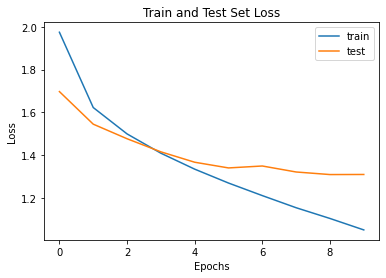
\includegraphics[width=8cm]{hw3/loss_plot.png}
        \centering
    \end{figure}
    
    \item \textbf{Evaluate: To evaluate your model, compute the following metrics on the train and test set, including them in your write-up. For each of the following metrics, use the model's "hard assignment" of labels, i.e. your model's predictions should assign each data point to only 1 class:
    \begin{itemize}
        \item The model's classification accuracy
        \item The model's precision and recall for each of the 10 classes
        \item What kinds of errors do you believe that the trained model is making? Use evidence (such as the above metrics, example misclassified images, or any other metrics of your choice) to support your claims.
        \item Include in your submission: train/test accuracy, train/test precision/recall for 10 classes, and evidence to support your hypothesis about the model's errors.
    \end{itemize}}
    
    
    Using the definitions of precision and recall:
    $$
        \text{Precision} = \frac{\text{True Positive}}{\text{True Positive} + \text{False Positive}}
    $$  
    $$
        \text{Recall} = \frac{\text{True Positive}}{\text{True Positive} + \text{False Negative}}
    $$  
    
    \textbf{Training Set} \\
    The overall model classification \textbf{accuracy} is $64\%$\\
	Precision for class 0 plane : 59.8 \% \\
    Recall for class 0 plane : 58.9 \% \\
    Precision for class 1 car : 64.3 \% \\
    Recall for class 1 car : 65.2 \% \\
    Precision for class 2 bird : 44.51 \% \\
    Recall for class 2 bird : 40.5 \% \\
    Precision for class 3 cat : 35.29 \% \\
    Recall for class 3 cat : 36.1 \% \\
    Precision for class 4 deer : 48.32 \% \\
    Recall for class 4 deer : 46.0 \% \\
    Precision for class 5 dog : 46.49 \% \\
    Recall for class 5 dog : 41.0 \% \\
    Precision for class 6 frog : 53.65 \% \\
    Recall for class 6 frog : 64.7 \% \\
    Precision for class 7 horse : 63.24 \% \\
    Recall for class 7 horse : 59.0 \% \\
    Precision for class 8 ship : 62.36 \% \\
    Recall for class 8 ship : 71.4 \% \\
    Precision for class 9 truck : 60.21 \% \\
    Recall for class 9 truck : 57.2 \% \\
    
    \textbf{Testing Set} \\
    The overall model classification \textbf{accuracy} is $67\%$\\
    Precision for class 0 plane : 69.72 \% \\
    Recall for class 0 plane : 63.1 \% \\
    Precision for class 1 car : 77.0 \% \\
    Recall for class 1 car : 65.6 \% \\
    Precision for class 2 bird : 53.36 \% \\
    Recall for class 2 bird : 46.0 \% \\
    Precision for class 3 cat : 49.78 \% \\
    Recall for class 3 cat : 33.9 \% \\
    Precision for class 4 deer : 50.28 \% \\
    Recall for class 4 deer : 54.8 \% \\
    Precision for class 5 dog : 53.4 \% \\
    Recall for class 5 dog : 54.2 \% \\
    Precision for class 6 frog : 62.15 \% \\
    Recall for class 6 frog : 78.8 \% \\
    Precision for class 7 horse : 60.49 \% \\
    Recall for class 7 horse : 74.4 \% \\
    Precision for class 8 ship : 71.13 \% \\
    Recall for class 8 ship : 77.1 \% \\
    Precision for class 9 truck : 67.72 \% \\
    Recall for class 9 truck : 68.6 \% \\
    
    Across the test dataset these were the top 5 highest class to class occurrences of an incorrect prediction:
    \textbf{Top 5 Class Confusion counts:}\\
    Class 3 to class 5: 225 \\
    Class 5 to class 3: 180 \\
    Class 1 to class 9: 169 \\
    Class 6 to class 3: 156 \\
    Class 8 to class 0: 143 \\
    Class 9 to class 1: 138 \\

    The model seems to be mainly making mis-classification errors between Cats and dogs, cars and trucks. This is likely due to the classifier using information from the color similarity of the images, cars and trucks, and dogs and cats share similar color and positional information.\\
    Intuitively this makes sense as the model is taking each value of color and position as equally important - pictures with large amounts of the same color in the same position will be harder to differentiate.
    
    \item \textbf{Explore: Create a new neural network with at least 1 architectural modification. Some things you can explore are adding or removing layers, changing the number of nodes at each layer, or experimenting with convolutional and pooling layers (see Appendix). The only requirement is that your model attain at least 50\% test set accuracy after training for 10 epochs. This part of the problem is intentionally open-ended, and we encourage you to explore!
    For your new neural network, include a plot of train and test set loss in your writeup. Calculate your model's train/test accuracy and precision/recall for the 10 classes.\\
    In your writeup, copy and paste your modified neural network class and describe the architectural changes you made. Write at least 1 sentence about why you hypothesize your new neural network performed better or performed worse than the network in Part 3.4. \\
    Include in your submission: Your neural network class code, 1 plot of train/test loss, metrics from Part 3.6 for this new neural net, and explanation of performance.}
    
    For this problem I added two convolution layers to my existing network, this involves applying pooling functions after the convolution layers. I then altered the layer parameters until the network started to predict well. 
    
    \textbf{Neural Network Class:}
    \begin{lstlisting}
    class Part7NeuralNetwork(nn.Module):
        def __init__(self):
            
            super(Part7NeuralNetwork, self).__init__()
            self.conv1 = nn.Conv2d(3, 10, 5)
            self.pool = nn.MaxPool2d(2, 2)
            self.conv2 = nn.Conv2d(10, 16, 5)
            self.fc1 = nn.Linear(16 * 5 * 5, 110)
            self.fc2 = nn.Linear(110, 80)
            self.fc3 = nn.Linear(80, 10)
    
        def forward(self, x):
            # Pool results from layers 1 and 2
            x = self.pool(F.relu(self.conv1(x)))
            x = self.pool(F.relu(self.conv2(x)))
            # Reshape the array
            x = x.view(-1, 16 * 5 * 5)
            # Apply relu functions
            x = F.relu(self.fc1(x))
            x = F.relu(self.fc2(x))
            x = F.relu(self.fc3(x))
            return x
    \end{lstlisting}
    
    \begin{figure}[H]
        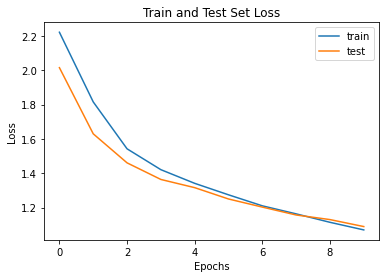
\includegraphics[width=8cm]{hw3/loss_plot3.7.png}
        \centering
    \end{figure}
    
    \textbf{Training Set} \\
    The overall model classification \textbf{accuracy} is $64\%$\\
    Precision for class 0 plane : 71.99 \% \\
    Recall for class 0 plane : 65.64 \% \\
    Precision for class 1 car : 80.44 \% \\
    Recall for class 1 car : 69.48 \% \\
    Precision for class 2 bird : 55.57 \% \\
    Recall for class 2 bird : 49.76 \% \\
    Precision for class 3 cat : 52.42 \% \\
    Recall for class 3 cat : 35.96 \% \\
    Precision for class 4 deer : 53.57 \% \\
    Recall for class 4 deer : 60.1 \% \\
    Precision for class 5 dog : 54.71 \% \\
    Recall for class 5 dog : 55.74 \% \\
    Precision for class 6 frog : 63.29 \% \\
    Recall for class 6 frog : 77.2 \% \\
    Precision for class 7 horse : 63.54 \% \\
    Recall for class 7 horse : 75.36 \% \\
    Precision for class 8 ship : 74.35 \% \\
    Recall for class 8 ship : 79.06 \% \\
    Precision for class 9 truck : 70.86 \% \\
    Recall for class 9 truck : 73.2 \% \\

    \textbf{Testing Set} \\
    The overall model classification \textbf{accuracy} is $61\%$\\
    Precision for class 0 plane : 69.72 \% \\
    Recall for class 0 plane : 63.1 \% \\
    Precision for class 1 car : 77.0 \% \\
    Recall for class 1 car : 65.6 \% \\
    Precision for class 2 bird : 53.36 \% \\
    Recall for class 2 bird : 46.0 \% \\
    Precision for class 3 cat : 49.78 \% \\
    Recall for class 3 cat : 33.9 \% \\
    Precision for class 4 deer : 50.28 \% \\
    Recall for class 4 deer : 54.8 \% \\
    Precision for class 5 dog : 53.4 \% \\
    Recall for class 5 dog : 54.2 \% \\
    Precision for class 6 frog : 62.15 \% \\
    Recall for class 6 frog : 78.8 \% \\
    Precision for class 7 horse : 60.49 \% \\
    Recall for class 7 horse : 74.4 \% \\
    Precision for class 8 ship : 71.13 \% \\
    Recall for class 8 ship : 77.1 \% \\
    Precision for class 9 truck : 67.72 \% \\
    Recall for class 9 truck : 68.6 \% \\
    
    
    \textbf{Top 5 Class Confusion counts:}\\
    Class 6 to class 9: 24 \\
    Class 7 to class 0: 22 \\
    Class 8 to class 2: 21 \\
    Class 6 to class 7: 21 \\
    Class 5 to class 6: 21 \\
    Class 4 to class 1: 21 \\
    
    I think this neural network performed better than before because it was using smaller pieces of the images to determine similarity. This forces the classifier to compare things like edge shapes rather than background color as the small subsection of the image may not have any background color in it. However, the horse class still looks to be quite a tricky one to differentiate as it is still being confused with Frogs. Even so, the confused classes are considerably more evenly spread across each class to class pair, this means that the model is performing better as a generalized model without a specific weakness (like background color).
    
\end{enumerate}


\newpage
%%%%%%%%%%%%%%%%%%%%%%%%%%%%%%%%%%%%%%%%%%%%%
% Name and Calibration
%%%%%%%%%%%%%%%%%%%%%%%%%%%%%%%%%%%%%%%%%%%%%
\subsection*{Name}
Phil Labrum
\subsection*{Collaborators and Resources}
Tommy Maldonado\\
Natalie Margulies\\
Daniel Rodrigues\\

\subsection*{Calibration}
45-50 hrs

\end{document}
